\newpage
\section{Thực hành chung}
\subsection{Yêu cầu}
Thực hiện phép nhân ma trận với vector.
\subsection{Cơ sở toán học}
Phép nhân ma trận với vector là một phép toán phổ biến trong đại số tuyến tính.

Công thức tính toán như sau:
\[ \mathbf{w} = A \cdot \mathbf{v} \]

Trong đó:
\begin{itemize}
 \item Với \( A \) là ma trận có kích thước \( m \times n \).
 \item Với \( \mathbf{v} \) là vector có kích thước \( n \times 1 \).
 \item Với \( \mathbf{w} \) là vector kết quả có kích thước \( m \times 1 \).
\end{itemize}

Để tính giá trị của \( \mathbf{w} \), thực hiện các phép nhân và cộng tương ứng:
\[ \mathbf{w}_i = \sum_{j=1}^{n} A_{ij} \cdot v_j \]

Trong đó:
\begin{itemize}
 \item Với \( A_{ij} \) là phần tử ở hàng \( i \), cột \( j \) của ma trận \( A \).
 \item Với \( v_j \) là phần tử thứ \( j \) của vector \( \mathbf{v} \).
 \item Với \( \mathbf{w}_i \) là phần tử thứ \( i \) của vector kết quả \( \mathbf{w} \).
\end{itemize}

\textbf{Ví dụ:}
Cho ma trận \( A \) và vector \( \mathbf{v} \) sau:

\[ A = \begin{bmatrix} 1 & 2 & 3 \\ 4 & 5 & 6 \end{bmatrix}, \quad \mathbf{v} = \begin{bmatrix} 2 \\ 1 \\ 3 \end{bmatrix} \]

Phép nhân ma trận \( A \) với vector \( \mathbf{v} \) sẽ tạo ra vector \( \mathbf{w} \) như sau:

\[ \mathbf{w} = A \cdot \mathbf{v} \]

Công thức tính toán:

\[ \begin{bmatrix} w_1 \\ w_2 \end{bmatrix} = \begin{bmatrix} 1 & 2 & 3 \\ 4 & 5 & 6 \end{bmatrix} \cdot \begin{bmatrix} 2 \\ 1 \\ 3 \end{bmatrix} \]

Thực hiện phép nhân và cộng:

\[ w_1 = 1 \cdot 2 + 2 \cdot 1 + 3 \cdot 3 = 13 \]

\[ w_2 = 4 \cdot 2 + 5 \cdot 1 + 6 \cdot 3 = 31 \]

Do đó, vector kết quả \( \mathbf{w} \) là:

\[ \mathbf{w} = \begin{bmatrix} 13 \\ 31 \end{bmatrix} \]




\subsection{Mã nguồn phép nhân ma trận với vector}

\subsubsection{Mã nguồn lập trình tuần tự phép nhân ma trận với vector}
\begin{listing}[H]
 \centering
 \inputminted{cpp}{sources/MaNguon1TT.cpp}
 \caption{Mã nguồn lập trình tuần tự phép nhân ma trận với vector}
 \label{code:MaNguon1TT}
\end{listing}

\subsubsection{Mã nguồn lập trình song song phép nhân ma trận với vector}
\begin{listing}[H]
 \centering
 \inputminted{cpp}{sources/MaNguon1SS.cpp}
 \caption{Mã nguồn lập trình song song phép nhân ma trận với vector}
 \label{code:MaNguon1SS}
\end{listing}














\subsection{Kết quả:}
\subsubsection{Bảng kết quả phép nhân ma trận với vector}




 
\begin{table}[h] %!nghia
 \centering
 \begin{tabular}{|c|c|c|c|}
 
 \hline
 \multicolumn{3}{|c|}{\textbf{BẢNG KẾT QUẢ}} \\ 
 \hline
 \textbf{Kích thước} & \textbf{Thời gian lập trình tuần tự} & \textbf{Thời gian lập trình song song} \\ \hline
 11111111111111111 & 11111111111111111 & 11111111111111111 \\ \hline
 11111111111111111 & 11111111111111111 & 11111111111111111 \\ \hline
 11111111111111111 & 11111111111111111 & 11111111111111111 \\ \hline
 \end{tabular}

 \caption{ViDuBangThuong} %!nghia
 \label{table:nghia1} %!nghia
 \end{table} 
 
 
 
\subsubsection{Biểu đồ phép nhân ma trận với vector}

 
\begin{figure}[h] %!nghia
 \centering
 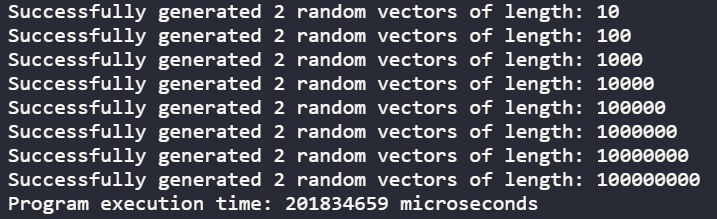
\includegraphics[width=1\textwidth]{pictures/image.png} %!nghia
 \caption{ViDuHinhAnhTheoChieuNgang} %!nghia
 \label{pictures:nghia12} %!nghia
 \end{figure} 
 

\subsection{Nhận xét}
\lipsum[1]


